\documentclass[tikz]{standalone}
\usetikzlibrary{calc,patterns,angles,quotes}
\usepackage{pgfplots}
\pgfplotsset{compat=newest}

\pagestyle{empty}

\begin{document}
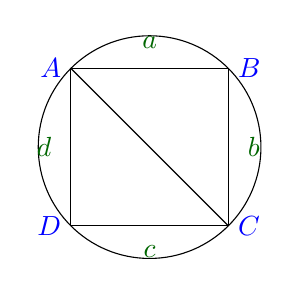
\begin{tikzpicture}
  \draw (1, 1) circle(1.414);
  \coordinate [label={[blue]left:$A$}] (A) at (0, 2);
  \coordinate [label={[blue]right:$C$}] (C) at (2, 0);
  \coordinate [label={[blue]right:$B$}] (B) at (2, 2);
  \coordinate [label={[blue]left:$D$}] (D) at (0, 0);
  \draw (B) -- (C);
  \draw (A) -- (B);
  \draw (C) -- (D);
  \draw (D) -- (A);
  \draw (C) -- (A);
  \node [label={[black!60!green]right :$b$}] at ( $ (B)!0.5!(C) $ ) () {};
  \node [label={[black!60!green]above:$a$}] at ( $ (A)!0.5!(B) $ ) () {};
  \node [label={[black!60!green]below:$c$}] at ( $ (C)!0.5!(D) $ ) () {};
  \node [label={[black!60!green]left:$d$}] at ( $ (D)!0.5!(A) $ ) () {};
\end{tikzpicture}
\end{document}
